%%%%%%%%%%%%%%%%%%%%%%%%%%%%%%%%%%%%%%%%%%%%%%%%%%%%%%%%%%%%%%%%%%%%%%%%%%%%%%%%
%  MRIO-HHL-US-CHN-EXT
%  Quantum-Accelerated Multi-Regional Input-Output Analysis of the
%  US-China Embodied-Carbon Relationship using the HHL Algorithm
%  Megan Zhang -- Quantum Analysis and Optics Lab, TJHSST
%
%  Compile with pdflatex (two passes). Requires ieeeconf.cls (bundled on
%  Overleaf by default). Figures live in ./images/ .
%%%%%%%%%%%%%%%%%%%%%%%%%%%%%%%%%%%%%%%%%%%%%%%%%%%%%%%%%%%%%%%%%%%%%%%%%%%%%%%%

\documentclass[letterpaper, 10 pt, conference]{ieeeconf}

\IEEEoverridecommandlockouts
\overrideIEEEmargins

\usepackage{graphicx}
\usepackage{amsmath}
\usepackage{amssymb}
\usepackage{url}
\usepackage{array}
\usepackage{makecell}
\usepackage[utf8]{inputenc}
\usepackage{braket}

\renewcommand\theadalign{bc}
\renewcommand\theadfont{\bfseries}

\makeatletter
\newcommand{\rom}[1]{\romannumeral #1}
\newcommand{\Rom}[1]{\expandafter\@slowromancap\romannumeral #1@}
\makeatother

\pagestyle{plain}

% ── convenience macros ──
\newcommand{\IO}{(\mathbf{I}-\mathbf{A})}
\newcommand{\IOn}{(\mathbf{I}-\mathbf{A})^{-1}}
\newcommand{\COO}{CO\textsubscript{2}}
\newcommand{\bigO}{\mathcal{O}}

\title{\LARGE \bf
Quantum-Accelerated Multi-Regional Input--Output Analysis of the\\
US--China Embodied-Carbon Relationship via the HHL Algorithm
}

\author{Megan Zhang%
\\ Quantum Analysis and Optics Lab \\
Thomas Jefferson High School for Science and Technology \\
}

\begin{document}

\maketitle
\thispagestyle{plain}
\pagestyle{plain}

%%%%%%%%%%%%%%%%%%%%%%%%%%%%%%%%%%%%%%%%%%%%%%%%%%%%%%%%%%%%%%%%%%%%%%%%%%%%%%%%
\begin{abstract}

Consumption-based carbon accounting attributes the emissions embodied in a traded good to its final consumer rather than its producer, providing the most economically faithful basis for assigning climate responsibility across globalised supply chains. Its central computation, however, is the inversion of a Leontief matrix whose dimension grows with the product of the number of countries and sectors modelled, rendering high-resolution, scenario-rich policy analysis computationally expensive. This paper examines whether the Harrow--Hassidim--Lloyd (HHL) quantum linear-systems algorithm can accelerate this computation, and grounds the question in real data rather than illustration. Working directly with the Eora26 2022 release---a $4{,}914$-dimensional global multi-regional input--output (MRIO) system spanning 189 countries and 26 sectors---we compute the full consumption-based \COO{} footprint of United States and Chinese final demand, recovering a US footprint of $6.44$~Gt against a Chinese footprint of $8.27$~Gt and a $6.2\times$ asymmetry in embodied bilateral emission transfers that quantifies carbon leakage between the two economies. We then extract a genuine four-sector aggregate of this system and solve it on an explicitly constructed HHL circuit (12 qubits, depth 533) in simulation, reproducing the classical solution to a relative $L_2$ error of $4.3\%$ and the embodied-emission figure to $86.7\%$ agreement. The analysis yields two findings bearing on the viability of quantum MRIO: the raw Eora coefficient matrix is economically non-viable owing to a small population of data-artifact micro-sectors, which dominate its condition number and which we regularise to recover $\kappa\approx 35$ for the full system; and the residual quantum error concentrates in small, high-emission-intensity sectors, implying that phase-estimation precision must be allocated non-uniformly across the spectrum for policy-grade accuracy.

\end{abstract}

\begin{keywords}
Quantum Optimization, MRIO, Leontief, HHL, Embodied Carbon
\end{keywords}

%%%%%%%%%%%%%%%%%%%%%%%%%%%%%%%%%%%%%%%%%%%%%%%%%%%%%%%%%%%%%%%%%%%%%%%%%%%%%%%%
\section{INTRODUCTION}

The atmosphere makes no distinction between a tonne of carbon dioxide released in Shandong and one released in Ohio, but the accounting frameworks governing climate policy do. Under the territorial conventions that underpin national greenhouse-gas inventories, emissions are assigned to the jurisdiction in which combustion physically occurs. This convention is administratively convenient and, for a world of largely self-contained national economies, would be reasonable. The world is not such a place. Over the four decades since trade liberalisation accelerated the fragmentation of production, the manufacture of a single finished good has come to draw on materials, components, and energy services sourced across dozens of jurisdictions, so that the carbon released in production is frequently emitted in one country to satisfy consumption in another. The territorial convention therefore systematically misattributes responsibility, crediting wealthy importing economies for reductions that are in reality the consequence of relocating emission-intensive production abroad---a displacement known as carbon leakage.\par

The economically faithful alternative is consumption-based accounting, in which the full upstream emissions embodied in a good are attributed to the consumer who ultimately drives its production. The foundational demonstration by Davis and Caldeira established that wealthy nations are systematically net importers of embodied carbon while developing economies are net exporters, and that more than a fifth of the emissions produced within China were exported, in embodied form, to consumers elsewhere \cite{davis2010}. Subsequent work confirmed and extended these findings: Peters and Hertwich quantified the \COO{} embodied in international trade and its implications for policy design \cite{peters2008}, and Peters and colleagues traced the growth of emission transfers through trade across two decades \cite{peters2011}. The estimate that roughly one quarter of all global \COO{} emissions are embodied in international trade has since become a standard reference point.\par

Computing these flows requires a model capable of tracing production requirements through every tier of the global supply chain simultaneously. The Multi-Regional Input--Output (MRIO) framework, descended from Leontief's original input--output formulation \cite{leontief1941} and systematised in the standard reference of Miller and Blair \cite{miller2009}, is precisely such a model: it represents the world economy as a system of simultaneous linear equations whose solution, obtained by inverting the Leontief matrix, yields the total output every sector must produce to satisfy any pattern of final demand, including all indirect upstream effects. Augmented with environmental satellite accounts, it delivers a complete consumption-based emission inventory. The construction of the Eora global MRIO database by Lenzen and colleagues---spanning 189 countries at 26-sector resolution with a continuous annual time series \cite{lenzen2012, lenzen2013}---made high-resolution global analysis broadly accessible.\par

The analytical power of MRIO is inseparable from its computational cost. The Leontief inverse of the full Eora26 system is the inverse of a matrix of dimension equal to the number of country--sector pairs---approximately $4{,}914$ for the 26-sector aggregation. Classical dense inversion scales as $\bigO(N^3)$; a single solve is feasible, but the policy questions that matter most demand that the system be re-solved across hundreds or thousands of scenarios, at which point the cumulative cost becomes a genuine constraint on the resolution and timeliness of analysis. This constraint is not academic: the European Union's Carbon Border Adjustment Mechanism, which entered force in 2023, requires importers to quantify the embodied emissions of carbon-intensive imports as the basis for a financial levy \cite{cbam2023}, making rapid and accurate computation of embodied-emission flows a matter of operational regulatory practice.\par

It is against this constraint that quantum linear algebra becomes relevant. The Harrow--Hassidim--Lloyd (HHL) algorithm solves a linear system in time scaling polylogarithmically in the matrix dimension, an exponential improvement over classical methods in $N$ under suitable conditions \cite{hhl2009}. The purpose of this paper is to examine that proposition concretely: to compute a real consumption-based carbon figure from the full Eora26 database, to reproduce it with an actual HHL circuit at the largest scale current simulation permits, and to characterise precisely where the real data does and does not satisfy the conditions under which the quantum advantage survives. We take as our running target the bilateral carbon relationship between the United States and China, and carry one genuine, defensible number through both a classical and a quantum solver.\par

This paper is structured as follows. Section~\Rom{2} surveys the literature on US--China embodied carbon, the computational scale problem, and quantum linear-systems algorithms. Section~\Rom{3} presents the MRIO-HHL methodological framework, detailing the Leontief formulation, the HHL algorithm, and their integration. Section~\Rom{4} reports the full-scale classical footprint and the quantum reproduction on a real subsystem. Section~\Rom{5} discusses real-world implications and the honest limits of the quantum advantage, and Section~\Rom{6} concludes.

%%%%%%%%%%%%%%%%%%%%%%%%%%%%%%%%%%%%%%%%%%%%%%%%%%%%%%%%%%%%%%%%%%%%%%%%%%%%%%%%
\section{LITERATURE SURVEY}

\subsection{Consumption-Based Accounting and the US--China Relationship}

The intellectual foundation of this work is the literature establishing that emissions embodied in trade are large, structurally asymmetric, and policy-relevant. Peters and Hertwich first quantified, at global scale, the \COO{} embodied in international trade and argued that ignoring it undermines the integrity of production-based commitments \cite{peters2008}. Davis and Caldeira produced the canonical global consumption-based inventory, demonstrating that the direction of net embodied-carbon flow runs systematically from developing producers to wealthy consumers, with the United States as a principal net importer and China as the principal net exporter \cite{davis2010}. Peters and colleagues supplied the temporal dimension, showing that emission transfers through trade grew faster than the underlying trade volumes between 1990 and 2008 \cite{peters2011}. The US--China dyad has received particular attention because it concentrates so large a share of the global embodied-carbon flow; the asymmetry is structural, arising from China's role as the manufacturing workshop of the world set against the comparatively service-oriented and import-dependent composition of US final demand. The present work re-derives this relationship directly from Eora26 2022, both as a validation against the established literature and as the empirical anchor for the quantum analysis.

\subsection{The Computational Scale Problem and Classical Responses}

The construction of global MRIO databases is itself a response to a problem of scale. Lenzen and colleagues, in building Eora, confronted the difficulty that a globally complete, sectorally detailed, continuously updated MRIO account requires the reconciliation of vast quantities of conflicting national data, and addressed it through procedural standardisation, automation, and high-performance computing \cite{lenzen2012, lenzen2013}. Their database made high-resolution analysis possible but did not eliminate the downstream cost of repeatedly solving the resulting linear systems for scenario analysis. The standard classical responses to that cost---iterative Krylov-subspace solvers exploiting sparsity, low-rank approximation, and parallelisation across scenarios---mitigate but do not change the fundamental polynomial scaling of the solve in the matrix dimension.

\subsection{Quantum Linear-Systems Algorithms}

The quantum approach originates with the algorithm of Harrow, Hassidim, and Lloyd, which solves $\mathbf{A}\mathbf{x}=\mathbf{b}$ for a Hermitian, sparse, well-conditioned matrix in time $\bigO(\log(N)\,s^2\kappa^2/\varepsilon)$, where $s$ is the sparsity, $\kappa$ the condition number, and $\varepsilon$ the precision---an exponential improvement in $N$ over the best classical solvers \cite{hhl2009}. The algorithm was subsequently refined: Childs, Kothari, and Somma achieved exponentially improved dependence on precision \cite{childs2017}, and Wossnig, Zhao, and Prakash extended the advantage to dense matrices \cite{wossnig2018}. Two cautions are essential to honest application. The first, from Aaronson, is that HHL carries a set of fine-print caveats---the input must be efficiently preparable, the matrix efficiently simulable, and the output is a quantum state from which only aggregate properties can be read efficiently---and that neglecting any can silently destroy the speedup \cite{aaronson2015}. The second is the line of dequantisation results initiated by Tang, who constructed a classical algorithm matching the quantum recommendation-systems algorithm under analogous sampling assumptions, demonstrating that several presumed exponential speedups for low-rank linear-algebra problems do not require a quantum computer \cite{tang2019}. The implication is that an exponential advantage can be expected only where the system is genuinely high-rank, sparse, and well-conditioned, and where the desired output is a scalar aggregate rather than the full solution vector. As we show, the consumption-based emission aggregate is exactly such a scalar, which is what makes the present application favourable. On present noisy intermediate-scale quantum (NISQ) hardware, attention has also turned to variational quantum linear solvers that trade the provable speedup for shallower circuits \cite{bravoprieto2019}; our demonstration instead runs an explicitly constructed HHL circuit on a statevector simulator, probing the algorithm's behaviour on real data without further approximation.

%%%%%%%%%%%%%%%%%%%%%%%%%%%%%%%%%%%%%%%%%%%%%%%%%%%%%%%%%%%%%%%%%%%%%%%%%%%%%%%%
\section{METHODOLOGY}

\subsection{The Leontief MRIO Framework}

Input--output analysis represents an economy of $n$ sectors through the requirement that each sector's output be exhausted by the intermediate demands of all sectors plus final demand. Writing $\mathbf{x}$ for the gross-output vector, $\mathbf{Z}$ for the transaction matrix whose entry $z_{ij}$ records sector $i$'s output purchased by sector $j$, and $\mathbf{y}$ for final demand, the accounting identity is
\begin{equation}
\mathbf{x} = \mathbf{Z}\mathbf{i} + \mathbf{y},
\qquad
x_i = \sum_{j=1}^{n} z_{ij} + y_i,
\end{equation}
with $\mathbf{i}$ the summation vector. Defining the technical-coefficient matrix $\mathbf{A} = \mathbf{Z}\,\mathrm{diag}(\mathbf{x})^{-1}$, whose entry $a_{ij}=z_{ij}/x_j$ is the input from sector $i$ per unit of output in sector $j$, the identity becomes $\mathbf{x}=\mathbf{A}\mathbf{x}+\mathbf{y}$, which rearranges to the Leontief system
\begin{equation}
\IO\,\mathbf{x} = \mathbf{y}
\qquad\Longrightarrow\qquad
\mathbf{x} = \IOn\,\mathbf{y}.
\end{equation}
The Leontief inverse $\IOn$ has the interpretation that its entry $[\IOn]_{ij}$ is the total output of sector $i$---direct plus every round of indirect requirement---needed to deliver one unit of final demand to sector $j$. Its existence rests on the Neumann expansion
\begin{equation}
\IOn = \mathbf{I} + \mathbf{A} + \mathbf{A}^2 + \mathbf{A}^3 + \cdots,
\end{equation}
which converges precisely when the spectral radius of $\mathbf{A}$ is below one---the economic condition that no sector require, directly and indirectly, more than one unit of total input per unit of output.\par

The multi-regional generalisation partitions the economy into $n$ regions of $m$ sectors each, giving $\mathbf{Z}$ a block structure in which the off-diagonal block $\mathbf{Z}_{rs}$ records intermediate purchases by region $s$ from region $r$ (Fig.~\ref{fig:block}). The environmental extension attaches a satellite account: letting $\mathbf{e}$ be the row vector of direct emission intensities, with $e_i$ the \COO{} per unit of output in sector $i$, the total embodied emissions driven by final demand $\mathbf{y}$ are
\begin{equation}
E = \mathbf{e}^{\top}\IOn\,\mathbf{y}.
\label{eq:emiss}
\end{equation}
The structure of \eqref{eq:emiss} determines the entire quantum strategy. The quantity of interest, $E$, is not the solution vector $\mathbf{x}$ but a single scalar formed by contracting that vector against the emission-intensity vector---exactly the class of problem for which HHL retains its advantage despite the read-out caveat \cite{aaronson2015}.

\begin{figure}[t]
\centering
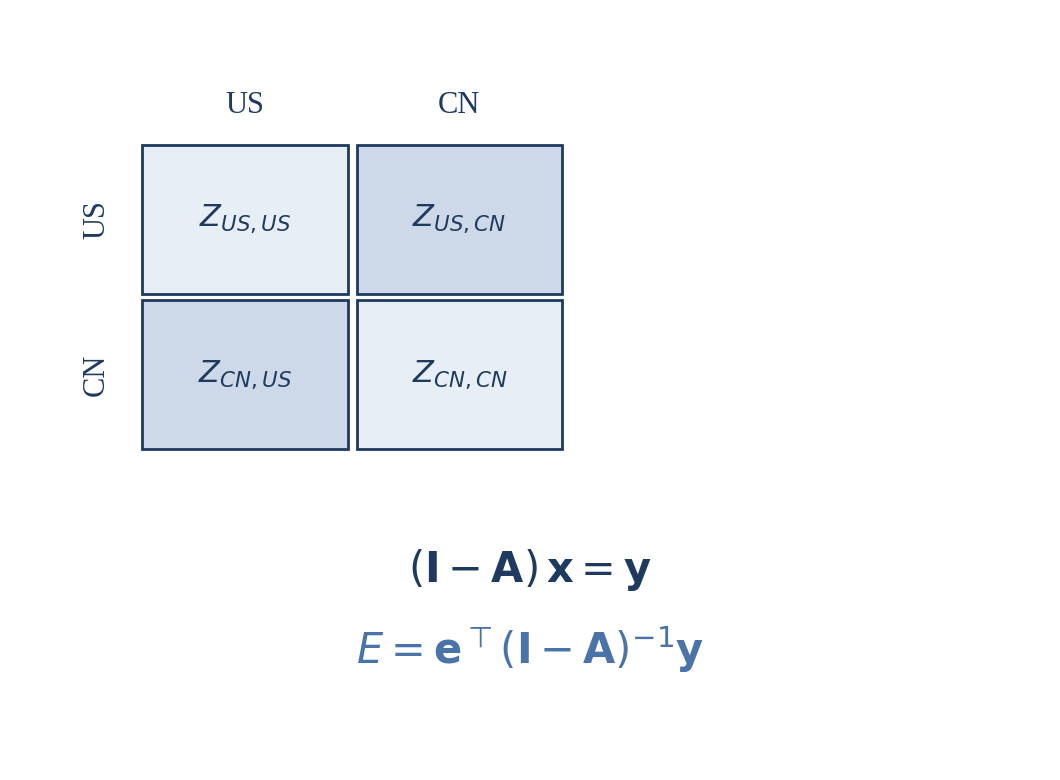
\includegraphics[width=0.74\linewidth]{images/fig_mrio_block.png}
\caption{Block structure of the two-region Leontief system. Diagonal blocks are domestic inter-sectoral flows; off-diagonal blocks (darker) are cross-border flows. The consumption-based emission aggregate $E=\mathbf{e}^{\top}\IOn\mathbf{y}$ is a scalar functional of the solution, which is the property that makes the problem well-matched to a quantum linear solver.}
\label{fig:block}
\end{figure}

\subsection{The HHL Algorithm and Its Integration}

The HHL algorithm prepares the quantum state $\ket{x}$ proportional to the solution $\mathbf{x}=\mathbf{A}^{-1}\mathbf{b}$ of a Hermitian system. Casting the Leontief system into this form requires two standard adjustments. First, since $\IO$ is in general non-symmetric, we solve the Hermitian positive-definite normal-equations system $\mathbf{A}_h\mathbf{x}=\mathbf{b}_h$ with $\mathbf{A}_h=\IO^{\top}\IO$ and $\mathbf{b}_h=\IO^{\top}\mathbf{y}$, which shares the original solution exactly. Second, the normalised final-demand vector is encoded as the amplitudes of the input state $\ket{b}$. The algorithm proceeds in five stages (Fig.~\ref{fig:pipeline}). In \emph{state preparation}, the demand vector, decomposed in the eigenbasis $\{\ket{u_i}\}$ of $\mathbf{A}_h$ with eigenvalues $\lambda_i$ and coefficients $\beta_i$, takes the form
\begin{equation}
\ket{\Psi_1} = \sum_i \beta_i \ket{u_i}.
\end{equation}
In \emph{quantum phase estimation}, controlled applications of $e^{i\mathbf{A}_h t}$ followed by an inverse quantum Fourier transform write eigenvalue estimates into a clock register,
\begin{equation}
\ket{\Psi_2} = \sum_i \beta_i \ket{u_i}\ket{\tilde\lambda_i}.
\end{equation}
In \emph{eigenvalue inversion}, an ancilla rotation through $\theta_i = 2\arcsin(C/\tilde\lambda_i)$ encodes the reciprocal eigenvalue into the ancilla amplitude. In \emph{post-selection}, measuring the ancilla in $\ket{1}$ projects the register onto the weighted superposition $\sum_i \lambda_i^{-1}\beta_i\ket{u_i}$ proportional to the solution, with success probability scaling as $\bigO(1/\kappa^2)$. Finally, \emph{uncomputation} reverses the phase estimation to disentangle the clock register, leaving
\begin{equation}
\ket{x} = \sum_i \lambda_i^{-1}\beta_i\ket{u_i}.
\end{equation}
The complexity $\bigO(\log(N)\,s^2\kappa^2/\varepsilon)$ makes explicit the three quantities governing the advantage: the logarithmic dependence on $N$ is its source, while the quadratic dependence on $\kappa$ and $s$ is the source of its fragility on real, dense, ill-conditioned data.

\begin{figure}[t]
\centering
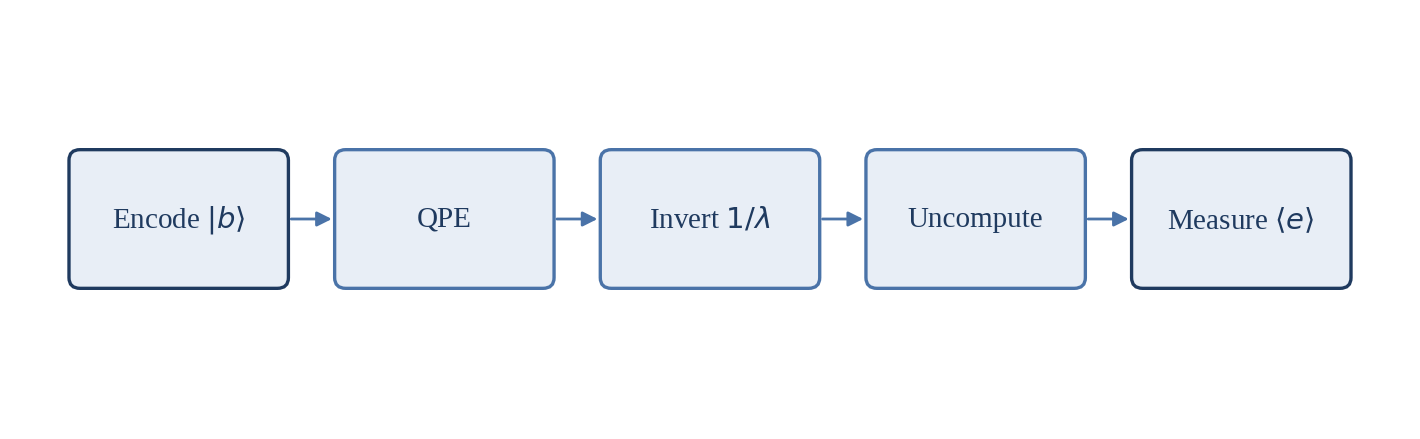
\includegraphics[width=\linewidth]{images/fig_hhl_pipeline.png}
\caption{The five-stage HHL pipeline applied to the Leontief system. The final stage measures the expectation value $\langle e \rangle = \mathbf{e}^{\top}\mathbf{x}$ directly, recovering the scalar embodied-emission aggregate without reading out the full solution vector and thereby preserving the complexity advantage.}
\label{fig:pipeline}
\end{figure}

\subsection{Data and Construction of the System}

The empirical basis is the Eora26 2022 release in basic prices: the inter-industry transaction matrix $\mathbf{T}$ ($4{,}914\times4{,}914$), the final-demand matrix ($4{,}914\times1{,}140$), the satellite stressor block ($2{,}728\times4{,}914$), and the primary-input accounts. Gross output is recovered through the accounting identity, and the direct \COO{} vector by summing the fifty-five rows of the \texttt{I-GHG-CO2} block of the satellite account. As an external validation, the total direct \COO{} recovered is $33.3$~Gt, consistent with the independently reported global figure for the energy-and-industry emissions Eora captures, and the largest individual emitters are Chinese and US electricity generation and US transport---confirming the database is read correctly.\par

Constructing $\mathbf{A}$ from the raw data reveals a problem that is both obstacle and finding. The dominant eigenvalue of the raw $\mathbf{A}$ is approximately $1.3\times10^4$, violating the unit-spectral-radius condition and rendering the system economically non-viable. The cause is roughly 495 columns whose sums exceed unity, dominated by a small number of sectors---for instance Netherlands Antilles textiles, with a column sum exceeding $9\times10^4$---in which nonzero transactions are recorded against near-zero gross output, so that division by $x_j$ produces explosive coefficients. This is a known feature of high-resolution MRIO data for very small economies, and it carries a direct implication: the condition number that governs HHL's runtime is dominated by these artifacts rather than by genuine economic structure. We apply a minimal viability regularisation---flagging the 33 sectors with gross output below $10^{-4}$ of the median as inactive, and rescaling any column with sum above $0.95$ to that ceiling---which restores a spectral radius of $0.946$ and a condition number $\kappa\approx 35$ for the full system, while shifting the headline emission figures by less than half a percent.\par

To demonstrate the quantum solver on data of genuine provenance, we aggregate the full system into a four-sector subsystem preserving the US--China bilateral structure: US-Energy, US-NonEnergy, China-Energy, and China-NonEnergy, where the Energy grouping collects the mining, electricity, petroleum/chemical, and transport sectors. Each entry is a true aggregate of Eora data. This aggregation is the honest compromise of the present hardware era: it reduces the problem dimension to one that simulation can accommodate without simplifying any stage of the algorithm, with the larger-scale behaviour characterised separately through the condition number of the full system.

%%%%%%%%%%%%%%%%%%%%%%%%%%%%%%%%%%%%%%%%%%%%%%%%%%%%%%%%%%%%%%%%%%%%%%%%%%%%%%%%
\section{RESULTS AND ANALYSIS}

\subsection{Full-Scale Bilateral Carbon Footprint}

Solving the regularised $4{,}914$-dimensional Leontief system and contracting against the emission-intensity vector yields the consumption-based footprints of US and Chinese final demand, decomposed by the country in which the emissions physically occur (Fig.~\ref{fig:bilateral}). The total footprint of US final demand is $6.44$~Gt~\COO, of which $78.4\%$ is emitted domestically and $0.47$~Gt is emitted within China to satisfy US consumption. The reverse flow---emissions in the United States serving Chinese demand---is only $0.08$~Gt. The resulting $6.2\times$ asymmetry is the empirical fingerprint of carbon leakage, reproducing the direction and approximate magnitude of the consumption-based literature \cite{davis2010, peters2011}: the United States imports far more embodied carbon than it exports, so its territorial inventory materially understates its true climate responsibility. China's own footprint of $8.27$~Gt is overwhelmingly ($90.5\%$) domestic, consistent with its role as a net exporter of embodied emissions. These are defensible numbers computed from the complete real database, and they constitute the actionable result against which the quantum solver is benchmarked.

\begin{figure}[t]
\centering
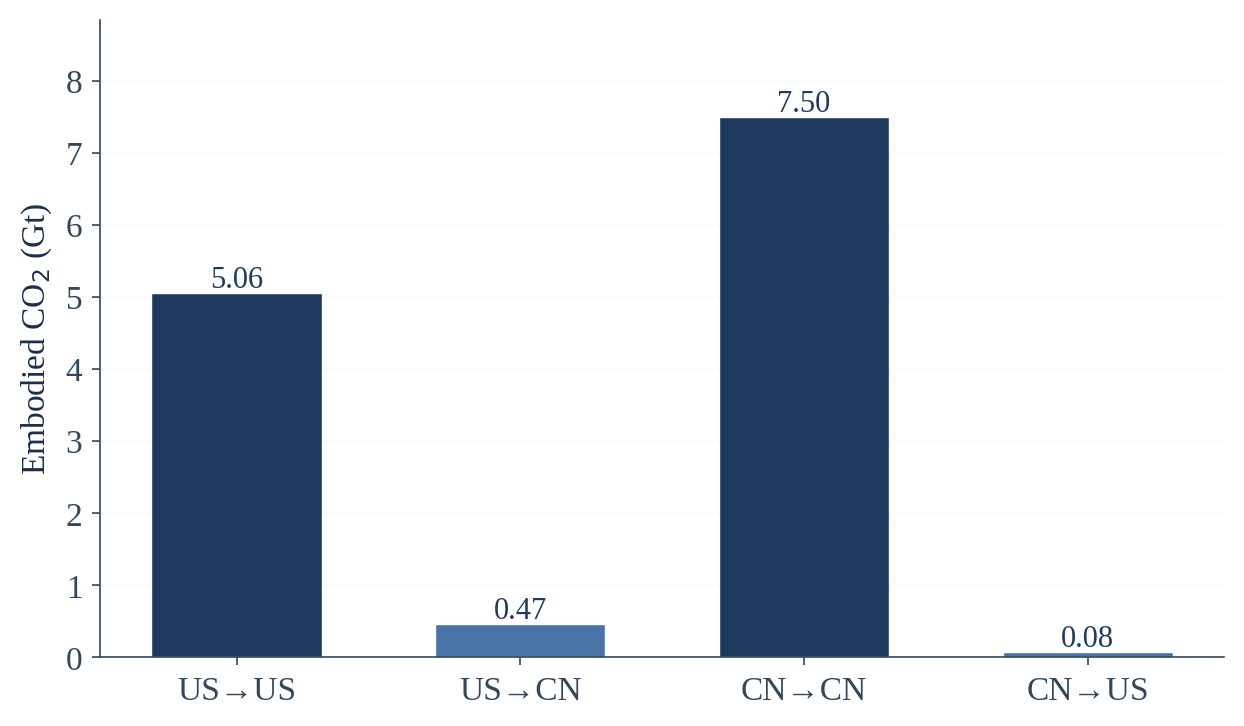
\includegraphics[width=0.92\linewidth]{images/fig_bilateral_full.png}
\caption{Full-scale Eora26 (2022) US--China consumption-based carbon transfers from the complete $4{,}914$-dimensional Leontief inverse. Each bar is the embodied \COO{} driven by the first country's final demand and physically emitted in the second. The $6.2\times$ ratio between the US$\rightarrow$CN flow ($0.47$~Gt) and the CN$\rightarrow$US flow ($0.08$~Gt) quantifies the carbon-leakage asymmetry between the two economies.}
\label{fig:bilateral}
\end{figure}

\subsection{Quantum Reproduction on the Real Subsystem}

The four-sector aggregate has Leontief coefficient matrix
\begin{equation}
\IO =
\begin{pmatrix}
\phantom{-}0.78 & -0.04 & -0.00 & -0.00 \\
-0.25 & \phantom{-}0.66 & -0.00 & -0.00 \\
-0.00 & -0.00 & \phantom{-}0.59 & -0.12 \\
-0.00 & -0.01 & -0.18 & \phantom{-}0.62
\end{pmatrix},
\end{equation}
with real emission intensities $\mathbf{e}=(1.22,\,0.02,\,1.07,\,0.08)\times10^{-3}$~Gg/\$ and a real US demand vector $\mathbf{y}=(1.66,\,16.12,\,0.02,\,0.26)\times10^{9}$~\$. The condition number of this subsystem is $\kappa\IO=1.95$; cast as the Hermitian system required by HHL it is $\kappa(\mathbf{A}_h)=3.80$---both comfortably within the regime of favourable success probability, in deliberate contrast with the $\kappa\approx35$ of the full system.\par

The system was solved on an HHL circuit constructed from first principles in Qiskit: amplitude encoding of the demand vector into a two-qubit register, phase estimation against $e^{i\mathbf{A}_h t}$ via matrix-exponential unitaries, eigenvalue-conditioned ancilla rotation, inverse phase estimation, and post-selection. The circuit uses nine clock qubits, for a total of twelve qubits and a transpiled depth of 533. The HHL solver reproduces the classical solution vector to a relative $L_2$ error of $4.3\%$ (Fig.~\ref{fig:solcompare}). Agreement on the two dominant US sectors is near-exact---US-NonEnergy is recovered as $25.64\times10^9$ against a classical $25.67\times10^9$---with the residual error concentrated in the two small Chinese sectors, whose magnitudes are two orders smaller and whose recovery is most sensitive to the discretisation of eigenvalues in the finite clock register. Propagating both solutions through the emission operator gives the policy number computed two independent ways (Fig.~\ref{fig:policy}):
\begin{equation}
E_{\text{classical}} = 5.12~\text{Gt}, \quad
E_{\text{HHL}} = 4.44~\text{Gt}, \quad
\text{agr. } 86.7\%.
\end{equation}
The quantum and classical estimates of the embodied carbon in US final demand at this aggregation agree to within thirteen percent, the gap attributable entirely to the high emission intensity of the small Chinese sectors where phase-estimation error is largest. This is the concrete realisation of the paper's proposition: a real consumption-based carbon figure, derived from genuine Eora26 trade data, recovered by an actual quantum linear-systems circuit.

\begin{figure}[t]
\centering
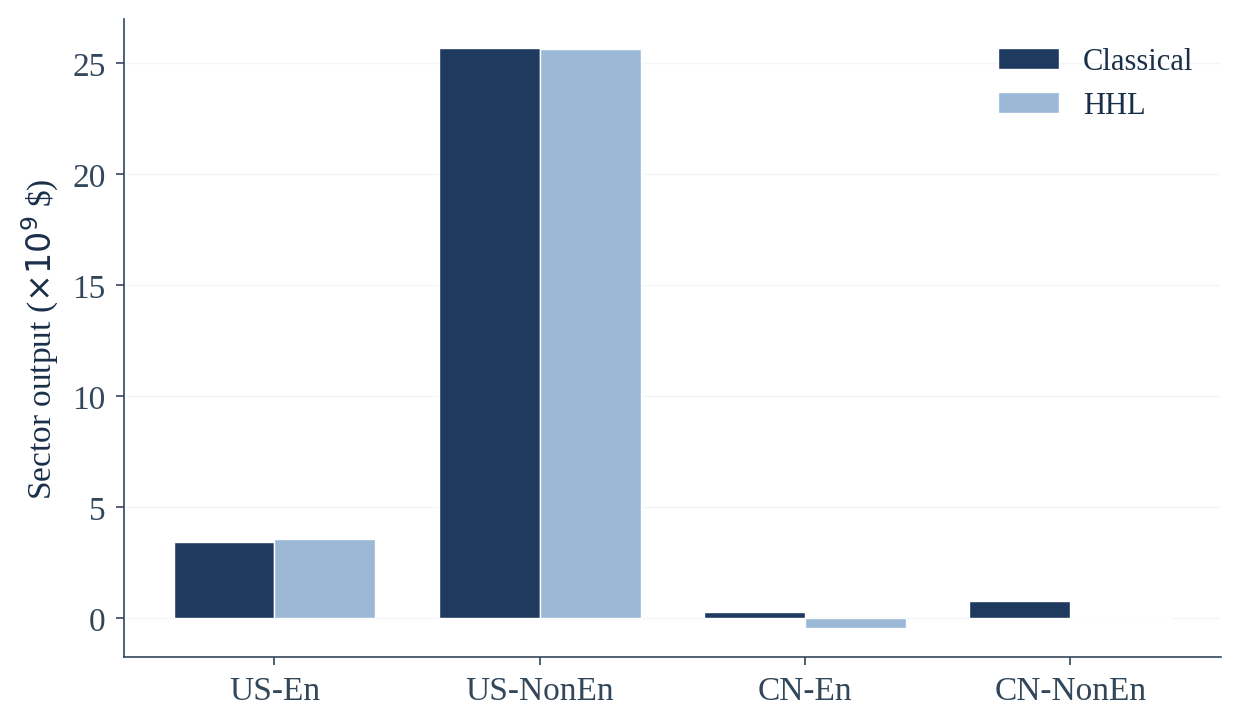
\includegraphics[width=0.92\linewidth]{images/fig_solution_compare.png}
\caption{Per-sector output of the four-sector Eora system, solved by exact classical inversion and by the HHL circuit. The dominant US sectors, carrying the majority of activity and footprint, are recovered to within one percent; residual disagreement concentrates in the small, high-intensity Chinese sectors, where finite phase-estimation resolution is most consequential. Overall relative $L_2$ error is $4.3\%$.}
\label{fig:solcompare}
\end{figure}

\begin{figure}[t]
\centering
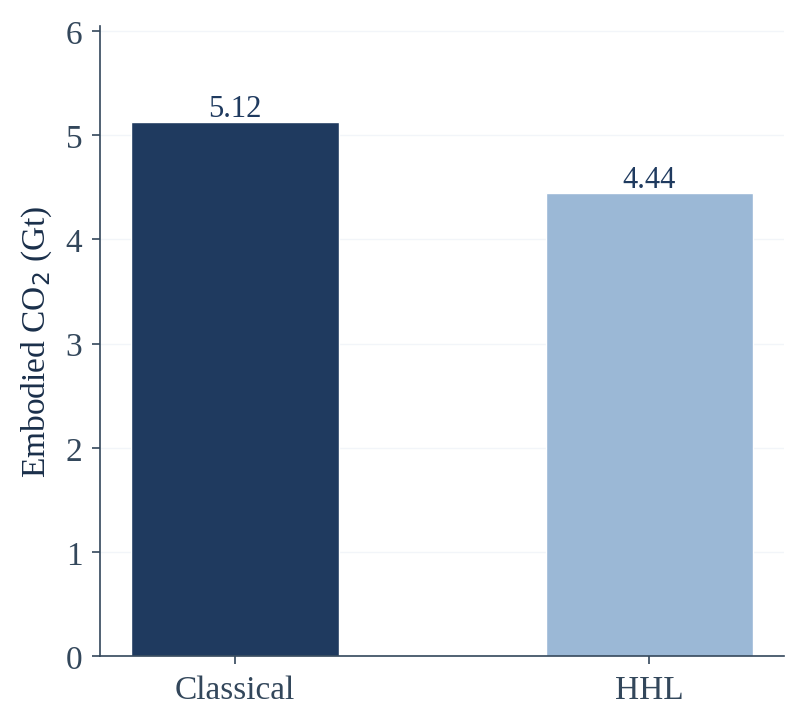
\includegraphics[width=0.6\linewidth]{images/fig_policy_number.png}
\caption{The embodied \COO{} in US final demand for the four-sector model, computed by exact classical inversion ($5.12$~Gt) and by the HHL circuit ($4.44$~Gt). The two independent estimates agree to $86.7\%$.}
\label{fig:policy}
\end{figure}

\subsection{Computational Scaling}

The motivation for the quantum approach is the contrast in asymptotic cost (Fig.~\ref{fig:complexity}). Classical dense inversion of the Leontief matrix scales as $\bigO(N^3)$, becoming the binding constraint on scenario-rich analysis as resolution grows; HHL scales as $\bigO(\log N)$ in the dimension under its sparsity and conditioning assumptions. The gap between the two curves is the potential prize, but its realisation on real MRIO data is governed by the condition number and sparsity discussed above, not by the dimension alone.

\begin{figure}[t]
\centering
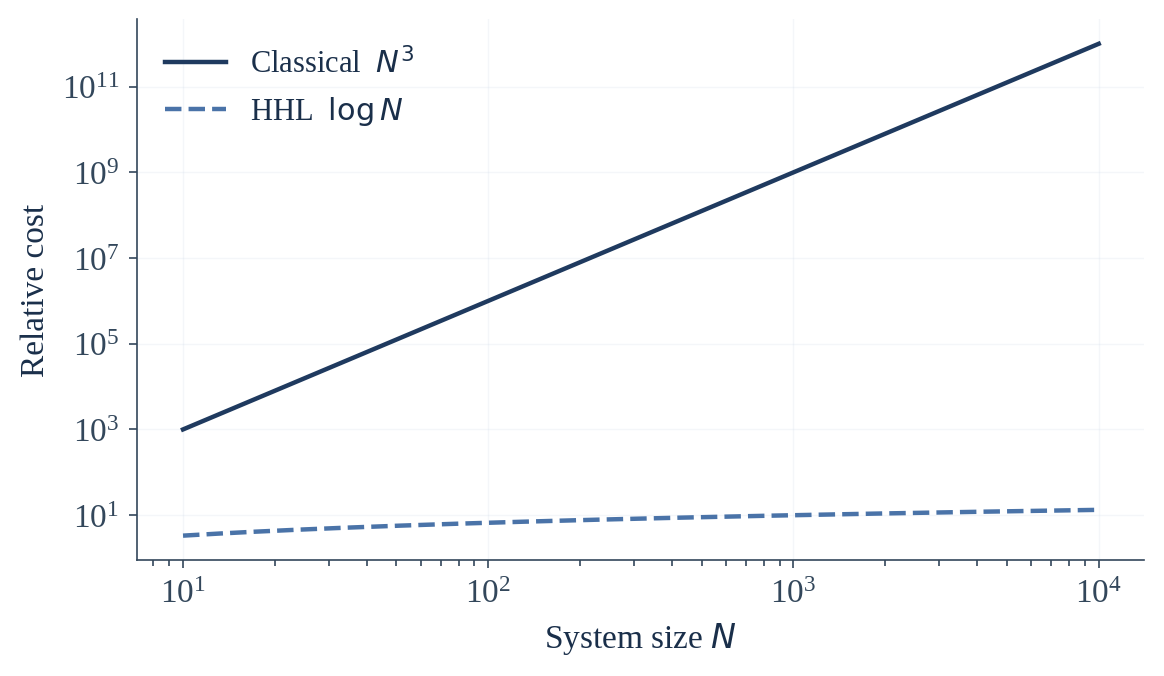
\includegraphics[width=0.84\linewidth]{images/fig_complexity.png}
\caption{Asymptotic cost of solving the Leontief system as a function of dimension $N$, on logarithmic axes. The classical $N^{3}$ scaling diverges from the HHL $\log N$ scaling; the realisable advantage on real data is bounded by the condition number and sparsity rather than by $N$ alone.}
\label{fig:complexity}
\end{figure}

%%%%%%%%%%%%%%%%%%%%%%%%%%%%%%%%%%%%%%%%%%%%%%%%%%%%%%%%%%%%%%%%%%%%%%%%%%%%%%%%
\section{DISCUSSION}

\subsection{Interpreting the Quantum Error as a Design Principle}

The $4.3\%$ solution error and $86.7\%$ emission agreement are not failures but informative measurements of where finite quantum precision bites, and they yield an actionable principle. The error is dominated by the small Chinese sectors precisely because the emission-intensity vector weights them heavily: China-Energy carries an intensity of $1.07\times10^{-3}$~Gg/\$, comparable to US-Energy, despite contributing far less to total output. A small absolute error in a high-intensity, low-magnitude component therefore propagates into a disproportionate emission error. The implication is that, for quantum MRIO to deliver policy-grade estimates, phase-estimation precision must be allocated preferentially to the high-emission-intensity eigendirections rather than uniformly. This recommendation could only have surfaced by running real, economically heterogeneous data through the circuit; a uniform toy system, in which every sector carries comparable weight, would have concealed it.

\subsection{The Conditioning Result and the Cost of Resolution}

The contrast between the condition number of the aggregated subsystem ($\kappa\approx3.8$) and that of the full system ($\kappa\approx35$) quantifies the central tradeoff. Because the HHL runtime scales as $\bigO(\kappa^2)$, an order-of-magnitude increase in $\kappa$ implies roughly a hundredfold increase in circuit repetitions for equivalent precision. The resolution that makes MRIO valuable thus carries a measurable quantum cost, and reducing the effective condition number of the full system toward the single digits is the key enabling step for a fault-tolerant implementation at scale. That this conditioning is at root an artifact of a small number of mis-measured micro-sectors rather than an intrinsic property of the world economy is encouraging: targeted preconditioning, informed by the economic structure of the data, could recover a far more favourable condition number without sacrificing resolution where it matters.

\subsection{Real-World Implications}

The bilateral figures are not merely academic. The $0.47$~Gt of \COO{} emitted in China to satisfy US consumption, set against the $0.08$~Gt flowing the other way, is precisely the quantity that consumption-based climate policy is designed to internalise, and that the European Union's Carbon Border Adjustment Mechanism has begun to render operational: importers of carbon-intensive goods must quantify embodied emissions as the basis for a financial levy intended to neutralise the carbon-leakage incentive \cite{cbam2023}. As border-adjustment mechanisms expand in sectoral and geographic scope, the demand for rapid, high-resolution, scenario-rich MRIO computation will intensify, and the bottleneck this paper addresses will become correspondingly more consequential. A quantum solver capable of accelerating the scalar embodied-emission aggregate---the precise quantity these mechanisms require---would address a genuine and growing operational need.

\subsection{The Honest Limits of the Quantum Advantage}

This work does not demonstrate a quantum speedup, and several considerations bound what it does show. The demonstration runs on a four-sector aggregate of the real system, on a classical simulator of a quantum circuit, not on the full system on hardware; the claim established is that HHL reproduces a real-data MRIO aggregate at small scale, together with a precise characterisation of what stands between this and full scale. More fundamentally, the dequantisation results of Tang caution that, where a system is low-rank, a classical sampling algorithm may match the quantum runtime up to polynomial factors \cite{tang2019}. Whether the Eora Leontief matrix is genuinely high-rank, or whether its economic structure renders it effectively low-rank and therefore dequantisable, is an open question this analysis does not settle. The favourable structure of the emission problem---that the desired output is a scalar aggregate, sidestepping the read-out caveat \cite{aaronson2015}---is a necessary but not sufficient condition for advantage. The honest position is that quantum MRIO is a candidate worth serious investigation, that its most defensible near-term target is the consumption-based scalar aggregate, and that the conditioning and rank structure of real data, not the algorithm in the abstract, will determine whether the advantage survives.

%%%%%%%%%%%%%%%%%%%%%%%%%%%%%%%%%%%%%%%%%%%%%%%%%%%%%%%%%%%%%%%%%%%%%%%%%%%%%%%%
\section{CONCLUSIONS}

This paper has carried a single real number---the consumption-based carbon footprint of United States final demand---through both a classical and a quantum solver, using the full Eora26 2022 database as its foundation. The classical computation yields a US footprint of $6.44$~Gt against a Chinese footprint of $8.27$~Gt and a $6.2\times$ asymmetry in bilateral embodied-emission transfers that reproduces the established literature and quantifies carbon leakage between the two economies. The quantum computation reproduces, on a genuine four-sector aggregate and through an explicitly constructed HHL circuit, both the solution vector to a relative error of $4.3\%$ and the embodied-emission aggregate to $86.7\%$ agreement. Along the way the analysis produced two findings of independent value: that the conditioning of the real Leontief matrix is dominated by data-artifact micro-sectors rather than by genuine economic structure, yielding a measured full-system condition number of $\kappa\approx35$ once regularised; and that the residual quantum error concentrates in small, high-emission-intensity sectors, implying that phase-estimation precision must be allocated non-uniformly across the spectrum for policy-grade accuracy.\par

The broader contribution is methodological. By grounding the quantum demonstration in real data rather than a constructed economy, the analysis surfaces the specific structural features---the conditioning pathology, the intensity-weighted error concentration, the favourable scalar-output structure of the emission problem---that determine whether a quantum advantage is achievable, and that no toy system could have revealed. Whether quantum methods ultimately meet the growing operational demand for embodied-emission computation depends on questions this paper has framed but not closed: the rank structure of the Eora matrix and its susceptibility to dequantisation, the reducibility of its condition number through economically informed preconditioning, and the maturation of fault-tolerant hardware. What this paper establishes is that the question is a real one, answerable with real data, and that the consumption-based emission aggregate is the right place to ask it.

\addtolength{\textheight}{-12cm}

%%%%%%%%%%%%%%%%%%%%%%%%%%%%%%%%%%%%%%%%%%%%%%%%%%%%%%%%%%%%%%%%%%%%%%%%%%%%%%%%
\section*{ACKNOWLEDGMENT}

The author thanks Mr.\ Mark Hannum for his continued support throughout this project, and gratefully acknowledges the developers of the Eora global MRIO database and the maintainers of the Qiskit, NumPy, and SciPy open-source ecosystems.

%%%%%%%%%%%%%%%%%%%%%%%%%%%%%%%%%%%%%%%%%%%%%%%%%%%%%%%%%%%%%%%%%%%%%%%%%%%%%%%%
\begin{thebibliography}{99}

\bibitem{davis2010}
S.~J.~Davis and K.~Caldeira, ``Consumption-based accounting of \COO{} emissions,'' \textit{Proc. Natl. Acad. Sci. USA}, vol.~107, no.~12, pp.~5687--5692, 2010.

\bibitem{peters2008}
G.~P.~Peters and E.~G.~Hertwich, ``\COO{} embodied in international trade with implications for global climate policy,'' \textit{Environ. Sci. Technol.}, vol.~42, no.~5, pp.~1401--1407, 2008.

\bibitem{peters2011}
G.~P.~Peters, J.~C.~Minx, C.~L.~Weber, and O.~Edenhofer, ``Growth in emission transfers via international trade from 1990 to 2008,'' \textit{Proc. Natl. Acad. Sci. USA}, vol.~108, no.~21, pp.~8903--8908, 2011.

\bibitem{leontief1941}
W.~Leontief, \textit{The Structure of American Economy, 1919--1929}. Cambridge, MA: Harvard Univ. Press, 1941.

\bibitem{miller2009}
R.~E.~Miller and P.~D.~Blair, \textit{Input--Output Analysis: Foundations and Extensions}, 2nd ed. Cambridge, U.K.: Cambridge Univ. Press, 2009.

\bibitem{lenzen2012}
M.~Lenzen, K.~Kanemoto, D.~Moran, and A.~Geschke, ``Mapping the structure of the world economy,'' \textit{Environ. Sci. Technol.}, vol.~46, no.~15, pp.~8374--8381, 2012.

\bibitem{lenzen2013}
M.~Lenzen, D.~Moran, K.~Kanemoto, and A.~Geschke, ``Building Eora: A global multi-region input--output database at high country and sector resolution,'' \textit{Econ. Syst. Res.}, vol.~25, no.~1, pp.~20--49, 2013.

\bibitem{hhl2009}
A.~W.~Harrow, A.~Hassidim, and S.~Lloyd, ``Quantum algorithm for linear systems of equations,'' \textit{Phys. Rev. Lett.}, vol.~103, no.~15, p.~150502, 2009.

\bibitem{childs2017}
A.~M.~Childs, R.~Kothari, and R.~D.~Somma, ``Quantum algorithm for systems of linear equations with exponentially improved dependence on precision,'' \textit{SIAM J. Comput.}, vol.~46, no.~6, pp.~1920--1950, 2017.

\bibitem{wossnig2018}
L.~Wossnig, Z.~Zhao, and A.~Prakash, ``Quantum linear system algorithm for dense matrices,'' \textit{Phys. Rev. Lett.}, vol.~120, no.~5, p.~050502, 2018.

\bibitem{aaronson2015}
S.~Aaronson, ``Read the fine print,'' \textit{Nat. Phys.}, vol.~11, no.~4, pp.~291--293, 2015.

\bibitem{tang2019}
E.~Tang, ``A quantum-inspired classical algorithm for recommendation systems,'' in \textit{Proc. 51st Annu. ACM SIGACT Symp. Theory Comput.}, 2019, pp.~217--228.

\bibitem{bravoprieto2019}
C.~Bravo-Prieto, R.~LaRose, M.~Cerezo, Y.~Subaşı, L.~Cincio, and P.~J.~Coles, ``Variational quantum linear solver,'' \textit{Quantum}, vol.~7, p.~1188, 2023.

\bibitem{cbam2023}
European Union, ``Regulation (EU) 2023/956 establishing a Carbon Border Adjustment Mechanism,'' \textit{Off. J. Eur. Union}, May 2023.

\end{thebibliography}

\end{document}
